%!TEX root = ../masters_thesis.tex

\section{Application} % (fold)
\label{sec:application}

HistoGlobe is a Web-based Historical Geographic Information System. The Data model and the conceptual model of the user interface were introduced in the first two sections of this chapter. This section introduces the underlying database model, a specific implementation of the data model, and the computational model that translates between the conceptual model and the database model of the system.

The first part provides an overview about the architecture of the system in section \ref{sub:system_architecture}.
% ... bla bla bla, the rest comes last
% problems
% - backward change: all Hivent Operations and Edit Operations are inversible :)
% - support uncertainty

% ------------------------------------------------------------------------------
\subsection{System Architecture} % (fold)
\label{sub:system_architecture}

HistoGlobe uses a classical client-server architecture of a Web-based information system. The user opens the application and interacts with it through the user interface in a Web browser, the \emph{client} side of the system. The Web \emph{server} is a remote computer that hosts the database and the middleware. The user interacts with the interface, the client-side application sends a request to the Web server for new data. The middleware checks the request and queries the necessary data from the database. It transforms the data and sends it back to the client. The interface shows the new information.

\begin{figure}[H]
  \vspace{1em}
  \centering
  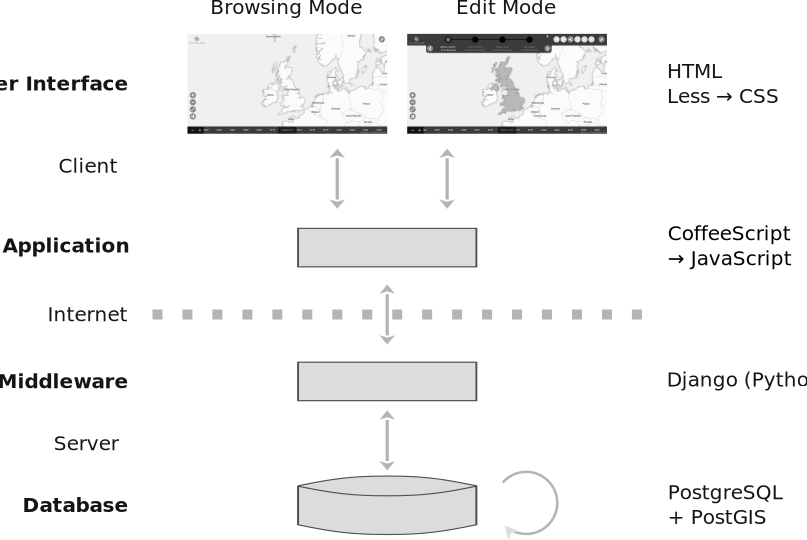
\includegraphics[width=0.7\textwidth]{graphics/development/system_architecture}
  \caption{The system architecture of HistoGlobe}
  \label{fig:system_architecture}
\end{figure}

This clear separation between the data, the application and the user interaction in this chapter and in the system follows directly from the \emph{model-view-controller} pattern: One part can be changed independently from the others parts: if the 2D map is replaced by a 3D globe, only the view changes, but the middleware and the database can stay untouched. Likewise, the implementation of a new database technology has no consequences to the view.

% subsection system_architecture (end)

% ------------------------------------------------------------------------------
\subsection{Hivent Database Model} % (fold)
\label{sub:database_model}

From the system point of view, the underlying data model explained in section \ref{sec:hivent_model} has to be implemented in a database model. HistoGlobe uses \emph{Django}, a free and open-source web framework
\footnote{
  \emph{Django},
  The Web framework for perfectionists with deadlines,
  URL: \url{https://www.djangoproject.com/},
  last access: 27.05.2016
},
combined with \emph{PostgreSQL}
\footnote{
  \emph{PostgreSQL:},
  The world's most advanced open source database,
  URL: \url{http://www.postgresql.org/},
  last access: 31.10.2015
}
, one of the most popular Object-Relational Database Management Systems introduced in section \ref{sub:object_relational_database_management_systems}, on the server-side of the system. This allows HistoGlobe to take advantage of object-oriented concepts in a stable and fast relational database. Since the database is using a lot of geospatial data, the \emph{PostGIS} is used as a spatial database extension for PostgreSQL
\footnote{
  \emph{PostGIS},
  Spatial and Geographic Objects for PostgreSQL,
  URL: \url{http://postgis.net/},
  last access: 27.05.2016
}.

With these tools at hand, the database model shown in figure \ref{fig:database_model_er} was developed. It is the final result of a highly iterative process that underwent many improvements and adpations to new requirements introduced in the Human Centered Design process. The model is structured in two parts covereign four different domains of the spatio-temporal model: The lower part describes the semantic, spatial and thematic domain of Areas and the upper part represents the temporal domain of Hivents that introduces changes to the Areas. It is the core of the spatio-temporal \emph{Hivent Database Model}.

\begin{figure}[ht]
  \centering
  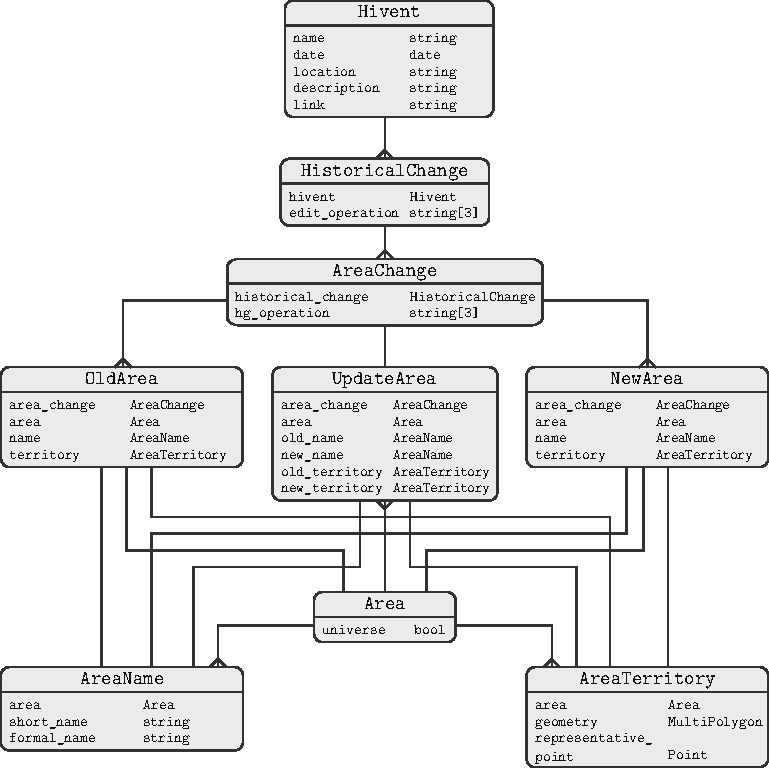
\includegraphics[width=0.8\textwidth]{graphics/development/database_model/er_model}
  \caption{The Hivent Database Model}
  \small{Each entity additionally has an \texttt{id} attribute, which is omitted for simplification purposes.}
  \label{fig:database_model_er}
\end{figure}

% - - - - - - - - - - - - - - - - - - - - - - - - - - - - - - - - - - - - - - -
\paragraph{Semantic, Spatial and Thematic Domain} % (fold)
\label{par:semantic_spatial_and_thematic_domain}

In the Hivent Model, the entity visible on the map is an Area with a name and a territory, as introduced in section \ref{sec:hivent_model}. In the database model, they are represented by three entities:

\begin{enumerate}
  \item \texttt{Area}: semantic domain defining the identity. The \texttt{universe} attribute is true for $\Omega$, for the other Areas it is false.
  \item \texttt{AreaTerritory}: spatial domain. A polypolygon describes the territories \texttt{geometry} and a \texttt{representative\_point} the position of the name label on the map.
  \item \texttt{AreaName}: thematic domain. It is defined by a \texttt{short\_name} and a \texttt{formal\_name}.
\end{enumerate}

% paragraph semantic_spatial_and_thematic_domain (end)

% - - - - - - - - - - - - - - - - - - - - - - - - - - - - - - - - - - - - - - -
\paragraph{Temporal Domain} % (fold)
\label{par:temporal_domain}

The main idea of the spatio-temporal data model is that the Areas can change over time. These changes are introduced by \texttt{Hivents}, the main entitity of the eponymic Hivent Database Model with five attributes: The \texttt{name} and a textual \texttt{description} of the Hivent, the point in time the Hvent happend (\texttt{date}), the Hivent \texttt{location} as a simple string and a \texttt{link} (URL) to the related article, serving as a historical source.

In the database, only valid time (\texttt{Hivent.date}) is taken into account, not database time. Each Hivent can introduce a set of \texttt{HistoricalChange}s that are described by one of the six high-level \texttt{edit\_operation}s introduced and understood by the user. Each \texttt{HistoricalChange} consists of a set of \texttt{AreaChange}s that represent one of the five low-level Hivent Operations (\texttt{hivent\_operation}). Each of them replaces a set of \texttt{OldArea}s with a set of \texttt{NewArea}s and might update the name or the territory of one specific \texttt{UpdateArea}.

% paragraph temporal_domain (end)

% - - - - - - - - - - - - - - - - - - - - - - - - - - - - - - - - - - - - - - -
\paragraph{Example} % (fold)
\label{par:example}

Figure \ref{fig:example_reunification} shows the Hivent Database Model at the example of the German Reunification on 3. October 1990. Before 1990, there were the Areas \texttt{GDR} (``German Democratic Republic'', East Germany) and \texttt{FRG} (``Federal Republic of Germany'', West Germany). A user introduced an historical change with a Merge operation (\texttt{MRG}) in the Edit Mode between \texttt{FRG} and \texttt{GDR}. The new Area received the short name ``Germany'' and the same formal name ``Federal Republic of Germany'' as previous West Germany. Internally, the Edit Mode translates this historical change to an \texttt{INC} of \texttt{GBDR} into \texttt{FRG} and a subsequent \texttt{NCH} of the \texttt{FRG}. One Area ceases, one Area is updated twice and no new Area is created.

\begin{figure}[ht]
  \vspace{1em}
  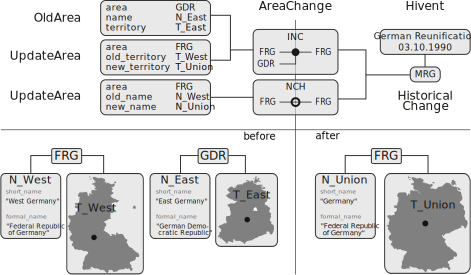
\includegraphics[width=0.9\textwidth]{graphics/development/database_model/example_reunification}
  \caption{Visualization of the German Reunification in the Hivent Database Model}
  \label{fig:example_reunification_2}
\end{figure}


% paragraph example (end)

% - - - - - - - - - - - - - - - - - - - - - - - - - - - - - - - - - - - - - - -
\paragraph{Initial Dataset} % (fold)
\label{par:initial_dataset}

Section \ref{sub:data_sources} explained the lack of data about historical countries. It is out of the scope of this thesis to create a large testing dataset with the historical countries in the world. The inital dataset consists of the following countries, their names, borders and historical events:

\begin{enumerate}
  \item 193 UN member states and 2 observer states were created with a \texttt{CRE} Edit Operation (\texttt{SEC} from the universe).
  \item 7 countries with limited international recognition (Kosovo, Transnistria, South Ossetia, Abkhazia, Nagorno-Karabakh, Somaliland and Sahrawi Arab Democratic Republic, see section \ref{par:un_non_members_with_limited_recognition}) were included. They were partially created by a \texttt{DIS} Edit Operation (\texttt{SEC} from their homeland) on the day of their declaration of independence.
\end{enumerate}

% paragraph initial_dataset (end)

% - - - - - - - - - - - - - - - - - - - - - - - - - - - - - - - - - - - - - - -
\paragraph{Middleware} % (fold)
\label{par:middleware}

The Django web framework provides \emph{view} classes as the middleware that receives requests from the client, processes them, queries the necessary data from the database and returns an \texttt{HttpResponse} back to the client. In the naive implementation of the system, the middleware provides only two views for the two use cases:

\begin{enumerate}
  \item \textbf{\texttt{get\_all}} is initially called by the client side on loading the web service. The server responds to this \texttt{HttpRequest} request with a object containing all information stored in the database. While this behaviour is not scalable, for the initial dataset it was sufficient: The data was loaded in 3.5 seconds.
  \item \textbf{\texttt{save\_historical\_change}} is called by the client after an Edit Operation has been completely created in the Edit Mode. In the last step, the client assembles the relevant data for the \texttt{HistoricalChange}: the associated \texttt{Hivent} and \texttt{AreaChange}s), data about each \texttt{OldArea}, \texttt{UpdateArea} and \texttt{NewArea}. The view checks the data for consistency and stores them in the database. The method returns to the client a confirmation and a set of final \texttt{id}s for the entities stored in the database.
\end{enumerate}

% paragraph middleware (end)

% - - - - - - - - - - - - - - - - - - - - - - - - - - - - - - - - - - - - - - -
consistency: how does git work?

Areas
  A   focused old Area
  Ai  other old Areas
  Bi  new Area(s)
  Ti  temporary Area(s) inserted before

Conflicts
  A)  automatic resolution (one obvious solution)
  S)  semi-automatic resolution (two definite alternatives)
  M)  manual resolution (empty land, obvious conflicts)


NCH
---

A ---O--- A

next operation to A
  id:   no possible conflict
  terr: no possible conflict
  name: possible conflict

  UNI -> A ceases
A)    => A: update \texttt{name} in \texttt{OldArea}

  SEP -> A ceases
A)    => A: update \texttt{name} in \texttt{OldArea}

  INC -> A updates only territory, not name
      => A: no conflict

  SEC -> A updates only territory, not name
      => A: no conflict

  NCH -> A can still be renamed
A)    -> A: update \texttt{old\_name} in \texttt{UpdateArea}


INC
---

T----|
A ---O--- A

next operation to A
  id:   no possible conflict
  terr: possible conflict
  name: no possible conflict

  UNI -> A cedes in UNI with larger territory
A)    => A: update \texttt{territory} in \texttt{OldArea}
A)    => B: update \texttt{territory} in \texttt{NewArea}
        => recursive update (treat as INC)

  SEP -> A separated in SEP with larger territory into Bi, but what about the rest of the larger territory?
      => Bi: keep as they are
A)    => A: separate into Bi, but for rest: empty land
M)      => CONFLICT! need to be resolved manually

  INC -> A incorporates B with larger territory
A)    => A: update \texttt{old\_territory} and \texttt{new\_territory} in \texttt{UpdateArea}
        => recursive update (treat as INC)

  SEC -> A cedes Bi in SEC with larger territory, T was not part of A before, will not be part of Bi now
A)    => A: update \texttt{old\_territory} and \texttt{new\_territory} in \texttt{UpdateArea}
        => recursive update (treat as INC)

  NCH -> A updates only name, not territory
      => no conflict


SEC
---

A ---O--- A
     |--- T

next operation to A
  id:   no possible conflict
  terr: possible conflict
  name: no possible conflict

  UNI -> A ceases, Ti not directly involved in UNI, but its territory
A)    => A: update \texttt{territory} in \texttt{OldArea}
S)    => CONFLICT! a) keep T or b) UNI together with Ai to B?
      -> if a)
-> A)   B: subtract Ti from \texttt{territory} in \texttt{NewArea}
          => recursive update (treat as SEC)
      -> if b)
-> A)   for each Ti: add to \texttt{OldArea}

  SEP -> A ceases into Bi but Ti covers territory of Bi in Ti
      => Bi: territory that is not covered by Ti: keep for now
S)    => CONFLICT! territory that is covered by Ti: a) keep Ti or b) keep Bi?
      -> if a)
-> A)   update \texttt{territory} of A in \texttt{OldArea}
        update \texttt{territory} of Bi in \texttt{NewArea}
        => recursive update (treat as SEC)
      -> if b)
->Hivent UNI A with Ti to Ts (simultaneous) before SEP
        replace \texttt{area} A by Ts in \texttt{OldArea}


  INC -> territory of A enlarges, Ti not directly involved in INC, but its territory
A)    => A: update \texttt{old\_territory} in \texttt{UpdateArea}
S)    => CONFLICT! a) keep Ti or b) INC together with Ai into A?
      -> if a)
-> A)   A: update \texttt{new\_territory} in \texttt{UpdateArea}
          => recursive update (treat as SEC)
      -> if b)
-> A)   for each Ti: add to \texttt{OldArea}

  SEC -> territory of A shrinks, Bi gets seceded, but covered by T
      => Bi: territory that is not covered by T: keep for now
S)    => CONFLICT! territory that is covered by Ti: a) keep Ti or b) keep Bi?
      -> if a)
-> A)   A: update \texttt{old\_territory} in \texttt{UpdateArea}
        A: update \texttt{new\_territory} in \texttt{UpdateArea}
          => recursive update (treat as SEC)
        Bi: update \texttt{territory} in \texttt{NewArea}
          => recursive update (treat as SEC)
      -> if b)
-> A)   add Hivent Operation INC of Ti into A before SEC

  NCH -> A updates only name, not territory
      => no conflict


UNI
---

A ---|
     O--- T
B ---|

next operation to A
  id:   possible conflict
  terr: possible conflict
  name: no possible conflict

  UNI -> A does not exist anymore to be unified, but can be be replaced by T
A)     => T: replace \texttt{area} A by T in \texttt{OldArea}
A)     => B: update \texttt{territory} in \texttt{NewArea}
        => recursive update of territory of B (treat as INC)

  SEP -> A does not exist anymore to be separated. If A is replaced by T in SEP, Bi get created, but what about the rest of the larger territory?
A)    => T: replace \texttt{area} A by T in \texttt{OldArea}
      => Bi: keep as they are
      => rest of T not covered by Bi: empty land
M)     => CONFLICT! need to be resolved manually

  INC -> A does not exist anymore to incorporate B, but can be replaced by T
A)    => T: replace \texttt{area} A by T in \texttt{UpdateArea},
          update \texttt{old\_territory} and \texttt{new\_territory}
        => recursive update of area A to T and territory (treat as UNI)

  SEC -> A does not exist anymore to secede Bi, but can be replaced by T in SEC
A)    => T: replace \texttt{area} A by T in \texttt{UpdateArea},
          update \texttt{old\_territory} and \texttt{new\_territory}
        => recursive update of area A to T and territory (treat as UNI)

  NCH -> A does not exist anymore to be renamed
A)    => delete NCH operation


SEP
---

     |--- T1
A ---O
     |--- T2

next operation to A
  id:   possible conflict
  terr: possible conflict
  name: no possible conflict

  UNI -> A does not exist anymore to be unified. Ti occupy exactly the same territory as A before.
      => a) keep Ti or b) UNI with Ai to B?
S)      => CONFLICT: need to be resolved by decision
        -> if a)
          => Ti: remove Ti from UNI
-> A)        B: update \texttt{territory} of B in \texttt{newArea}
              => recursively update territory of B (treat as SEC)
        -> if b)
-> A)     => Ti: for each Ti replace \texttt{area} A by Ti in \texttt{OldArea}

  SEP -> A does not exist anymore to be separated. Ti occupy exactly the same territory as A before that separated to Bi
S)    => CONFLICT! a) use Ti or b) use Bi?
        -> if a)
-> A)     remove SEP operation
        -> if b)
-> A)     add operation UNI of Ti to Ts (simultaneous) before SEP
          replace \texttt{area} A by Ts in \texttt{OldArea}

  INC -> A does not exist anymore to incorporate B. It is impossible to say if B should be incorporated into Ti
M)    => CONFLICT! need to be manually resolved

  SEC -> A does not exist anymore to secede from. T1 and T2 occupy exactly the same territory as A before
S)    => CONFLICT! a) keep Ti) or b) keep Bi
      -> if a)
-> A)    remove INC operation
      -> if b)
        it is impossible to say where Bi should secede from, since A does not exist anymore
-> M)    => CONFLICT! needs to be resolved manually

      -> secede both from T1 and T2, unify to new Area

  NCH -> A does not exist anymore to be renamed
A)    => delete NCH operation



% subsection database_model (end)

% ------------------------------------------------------------------------------
\subsection{Computational Model} % (fold)
\label{sub:computational_model}

Class diagram

HistoGlobe

SpatialDisplay -> Map

TimeController  <-> Timeline
                <-> NowMarker

HiventController                AreaController <->  AreasOnMap
HiventHandle                    AreaHandle
Hivent
HistoricalChange    AreaChange  Area
                                AreaName            AreaNameLayerOnMap
                                AreaTerritory       AreaTerritoryLayerOnMap

DatabaseInterface

EditMode -> EditOperation -> EditOperationStep
NewTerritoryTool* NewNameTool NewHiventBox
WorkflowWindow

HistoGraph

LabelManager*

important little utils
  Button, ButtonArea
  NumberInput, TextInput, TextInputArea
  Title
  Watermark
  DoublyLinkedList
  WithinTree
  Geometry -> Polypolygon -> Polygon -> Polyline -> Point

% % - - - - - - - - - - - - - - - - - - - - - - - - - - - - - - - - - - - - - - -
% \paragraph{Functional description} % (fold)
% \label{par:functional_description}

% Each Hivent Operation can be described by a mathematical function. The following symbols are used in the equations:

% \begin{addmargin}[1em]{0em}
% \begin{tabbing}
%   symbolxx \= description1xx \= description2 \kill
%   $A$ \> set of old Areas that were active before the Historical Change \\
%   $B$ \> set of new Areas that are created in the Historical Change \\
%   $n:$ \> $n \in \mathbb{N}, n>0$ \> total number of old respectively new Areas \\
%   $i:$ \> $i \in [\textbf{1} .. n]$ \> iterator for the current old respectively new Area \\
%   $A_0/B_0$ \>    the first old respectively new Area ($i \geq 1 \Rightarrow$ not $A_i/B_i$~!) \\
%   $A_i/B_i$ \>    the current old respectively new Area ($i \geq 1 \Rightarrow$ not $A_0/B_0$~!) \\
%   $A_i^T/B_i^T$ \>the new territory of the current Area (a polypolygon) \\
%   $A_i^N/B_i^N$ \>the new name of the current Area (short and formal name) \\
% \end{tabbing}
% \end{addmargin}

% \vspace{-2.5em}
% \begin{align*}
%   (B_0)                       &= UNI([A_1 .. A_i .. A_n], B_0^N) \\
%   (A_0)                       &= INC(A_0, [A_1 .. A_i .. A_n]) \\
%   ([B_1 .. B_i .. B_n])       &= SEP(A_0, [[B_1^T, B_1^N] .. [B_i^T, B_i^N] .. [B_n^T, B_n^N]]) \\
%   (A_0, [B_1 .. B_i .. B_n])  &= SEC(A_0, A_0^T, [[B_1^T, B_1^N] .. [B_i^T, B_i^N] .. [B_n^T, B_n^N]]) \\
%   (A_0)                       &= NCH(A_0, A_0^N)
% \end{align*}

% % paragraph functional_description (end)

% - - - - - - - - - - - - - - - - - - - - - - - - - - - - - - - - - - - - - - -
\paragraph{Pseudocode description} % (fold)
\label{par:pseudocode_description}

of the HG operations in an object-oriented manner. The existance of a class \texttt{Area} is assumed. Each \texttt{Area} object has the following member variables: a \texttt{name}, a \texttt{territory} and a list of historical \texttt{predecessors} and \texttt{successors}. Single capital letter variables (\texttt{A}/\texttt{B}) denote arrays of \texttt{Area} objects. Variables with a capital letter followed by a number or lowercase letter (e.g. \texttt{B0}) are single \texttt{Area} objects.

\begin{minipage}[t]{0.47\textwidth}
\begin{lstlisting}[language=pseudocode,
  caption=Unification]
FUNCTION UNI(A, B0_name)
  # create new territory
  B0_territory = NEW Geometry # empty
  FOREACH Ai IN A
    B0_territory.union(Ai.territory)
  # create new area
  B0 = NEW Area(B0_name, B0_territory)
  # establish historical relationships
  FOREACH Ai IN A
    Ai.successors.add(B0)
    B0.predecessors.add(A1)
  # return new area
  RETURN B0
\end{lstlisting}
\end{minipage}    % N.B. the % is very important
\hspace{3.0em}    % N.B. this must go in this line, no blank lines !!!
\begin{minipage}[t]{0.47\textwidth}
\begin{lstlisting}[language=pseudocode,
  caption=Incorporation]
FUNCTION INC(A0, A)
  # update old area with new territory
  temp_terr = NEW Geometry # empty
  FOREACH Ai IN A
    temp_terr.union(Ai.territory)
  A0.territory = temp_terr
  # establish historical relationships
  FOREACH Ai IN A
    Ai.successor.add(A0)
    A0.predecessor.add(A1)
  # return new area
  RETURN A0
\end{lstlisting}
\end{minipage}

\begin{minipage}[t]{0.47\textwidth}
\begin{lstlisting}[language=pseudocode,
  caption=Separation]
FUNCTION SEP(A0, B_data)
  # create each new Area
  B = []
  FOREACH Bi_data in B_data
    B.add(NEW Area(
      Bi_data.name, Bi_data.territory)
    )
  # establish historical relationships
  FOREACH Bi IN B
    A0.successors.add(Bi)
    Bi.predecessors.add(A0)
  # return new areas
  RETURN B

\end{lstlisting}
\end{minipage}    % N.B. the % is very important
\hspace{3.5em}    % N.B. this must go in this line, no blank lines !!!
\begin{minipage}[t]{0.47\textwidth}
\begin{lstlisting}[language=pseudocode,
  caption=Secession]
FUNCTION SEC(A0, A_territory, B_data)
  # update old area with new territory
  A0.territory = A_territory
  # create each new Area
  B = []
  FOREACH Bi_data in B_data
    B.add(NEW Area(
      Bi_data.name, Bi_data.territory)
    )
  # establish historical relationships
  FOREACH Bi IN B
    A0.successors.add(Bi)
    Bi.predecessors.add(A0)
  # return old and new areas
  RETURN [A0, B]

\end{lstlisting}
\end{minipage}

\vspace{-1.5em}
\begin{minipage}[t]{0.47\textwidth}
\begin{lstlisting}[language=pseudocode,
  caption=Name Change]
FUNCTION NCH(A0, A_name)
  # update old area with new name
  A0.name = A_name
  # return updated area
  RETURN A0

\end{lstlisting}
\end{minipage}

% paragraph pseudocode_description (end)


\paragraph{Execute Historical Change} % (fold)
\label{par:execute_historical_change}

execute function for all operations the same

% - - - - - - - - - - - - - - - - - - - - - - - - - - - - - - - - - - - - - - -
\begin{lstlisting}[language=pseudocode,
  caption=class HGOperation]
## member variables
old_areas = []          # Area
new_areas = []          # Area
update_name = {
  area :          null  # Area
  old_name :      null  # AreaName
  new_name :      null  # AreaName
}
update_territory = {
  area :          null  # Area
  old_territory : null  # AreaTerritory
  new_territory : null  # AreaTerritory
}

## main function
FUNCTION execute(direction)

  # hide old areas
  FOREACH old_area IN old_areas
    IF direction IS 1 # forward change
      old_area.hide()
    ELSE              # backward change
      old_area.show()

  # show new areas
  FOREACH new_area IN new_areas
    IF direction IS 1 # forward change
      new_area.show()
    ELSE              # backward change
      new_area.hide()

  # check if the area name is updated
  IF update_name.area
    IF direction IS 1 # forward change
      update_name.area.name = new_name
    ELSE              # backward change
      update_name.area.name = old_name
    update_name.area.update()

  # check if the area territory is updated
  IF update_territory.area
    IF direction IS 1 # forward change
      update_territory.area.territory = new_territory
    ELSE              # backward change
      update_territory.area.territory = old_territory

\end{lstlisting}

% paragraph execute_historical_change (end)

HistoGraph
\begin{lstlisting}[language=pseudocode,
  caption=plotting Areas on the HistoGraph,
  label=lst:histograph_plot]
FUNCTION plot(reference_area, plot_start_date, plot_end_date)
  # plot the current Area
  # logic is omitted

  # recursively plot in historically backward direction
  FOREACH predecessor IN reference_area.predecessors
    IF predecessor.end_date >= plot_start_date
      plot(predecessor)

  # recursively plot in historically forward direction
  FOREACH successor IN reference_area.successors
    IF successor.start_date <= plot_end_date
      plot(successor)
\end{lstlisting}

store Hivents in DoublyLinkedList

% \begin{figure}[ht]
%   \centering
%   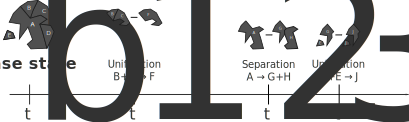
\includegraphics[width=0.8\textwidth]{graphics/basics/stdm/event-based_spatio-temporal_data_model}
%   \caption{The Event-Based Spatio-Temporal Data Model}
%   \label{fig:event-based_spatio-temporal_data_model}


A main problem is to maintain the integrity of the spatial topology when a new change gets inserted not at the end of the list. A simple example shows that problem: Given geo-object $X$ is part of the inital base configuration at change $t_b$. At a later change, e.g. $t_y$ $X$ gets replaced by object $Y$. If a new change that updates $X$ to $X'$ gets inserted before at time point $t_x < t_y$, then $t_y$ is not integer anymore, because object $X$ does not exist. That is why on insertion of a change, all succeeding changes have to be tested for integrity and it might be necessary to update later changes.


% subsection computational_model (end)

% section application (end)